%%%%%%%%%%%%%%%%%%%%%%%%%%%%%%%%%%%%%%%%%%%%%%%%%%%%%%%%%%%%%%%%%%%%%%
%%                     Process
%%%%%%%%%%%%%%%%%%%%%%%%%%%%%%%%%%%%%%%%%%%%%%%%%%%%%%%%%%%%%%%%%%%%%%

\subsection{Glyph: \glyph{Process}}
\label{sec:process}

A process is the basic process node in SBGN.  It describes a process that transforms a given set of biochemical entities---macromolecules, simple chemicals or unspecified entities---into another set of biochemical entities.  Such a transformation might imply modification of covalent bonds (conversion), modification of the relative position of constituents (conformational process) or movement from one compartment to another (translocation). A process transforms a set of entity pools (represented by \glyph{EPNs} in \SBGNPDLone) into another set of entity pools. A \glyph{process} is represented by a square box linked to two connectors, small arcs attached to the centers of opposite sides. The consumption (\sect{consumption}) and production (\sect{production}) arcs are linked to the extremities of those connectors. The modulatory arcs (\sect{arcs}) point to the other two sides of the box. A \glyph{process} connected to \glyph{production} arcs on opposite sides is a reversible process. 

\begin{figure}[H]
  \centering
  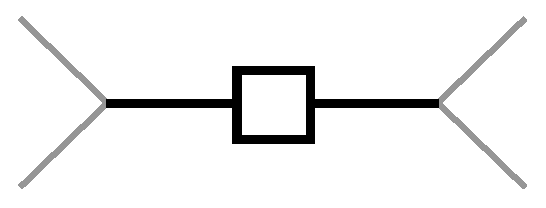
\includegraphics[scale = 0.4]{images/process}
  \caption{The \PD glyph for \glyph{process}.}
  \label{fig:process}
\end{figure}

